        %%******************************************%%
        %%                                          %%
        %%        Modello di tesi di laurea         %%
        %%            di Andrea Giraldin            %%
        %%                                          %%
        %%             2 novembre 2012              %%
        %%                                          %%
        %%******************************************%%

\begin{document}
    \frontmatter
    \begin{titlepage}
    \begin{center}
        \begin{LARGE}
            \textbf{\myUni}\\
        \end{LARGE}

        \vspace{10pt}

        \begin{Large}
            \textsc{\myDepartment}\\
        \end{Large}

        \vspace{10pt}

        \begin{large}
            \textsc{\myFaculty}\\
        \end{large}

        \vspace{30pt}
        \begin{figure}[htbp]
            \centering
            
\includegraphics[height=6cm]{unipd-logo}
        \end{figure}
        \vspace{30pt}

        \begin{LARGE}
            \textbf{\myTitle}\\
        \end{LARGE}

        \vspace{10pt}

        \begin{large}
            \textsl{\myDegree}\\
        \end{large}

        \vspace{40pt}

        \begin{large}
            \begin{flushleft}
                \textit{Relatore}\\
                \vspace{5pt}
                \profTitle\ \myProf
            \end{flushleft}

            % You can tweak the spacing to have professor and student names on the same line
            % useful if the page is broken by a long thesis title and you need more space
            % \vspace{-52pt}

            \begin{flushright}
                \textit{Laureando}\\
                \vspace{5pt}
                \myName \\
                \vspace{5pt}
                \textit{Matricola} \myID
            \end{flushright}
        \end{large}

        \vspace{40pt}

        \line(1, 0){338} \\
        \begin{normalsize}
            \textsc{Anno Accademico \myAA}
        \end{normalsize}
    \end{center}
\end{titlepage}

    \clearpage
\phantomsection
\thispagestyle{empty}

\hfill
\vfill

\noindent\myName: \textit{\myTitle,}
\myDegree,
\textcopyright\ \myTime.

    \cleardoublepage
\phantomsection
\thispagestyle{empty}
\pdfbookmark{Dedica}{Dedica}

\vspace*{3cm}

\begin{center}
    If you really look closely, most overnight successes took a long time. \\ \medskip
    % Try not to become a man of success. Rather become a man of value. \\ \medskip --- Albert Einstein
    % Time waits for no one. \\ \medskip --- Unknown Author
    --- Steve Jobs
\end{center}

\medskip

\begin{center}
    Ai miei genitori
\end{center}

    \cleardoublepage
\phantomsection
\pdfbookmark{Sommario}{Sommario}
\begingroup
\let\clearpage\relax
\let\cleardoublepage\relax
\let\cleardoublepage\relax

\chapter*{Sommario}

Il presente documento descrive il lavoro svolto durante il periodo di stage, della durata di trecento ore, dal laureando Nicolò Pellegrinelli presso l'azienda Prorob S.r.l., con sede a Grisignano di Zocco (VI).\\
Il tirocinio si è sviluppato intorno allo studio dei metodi di autenticazione e autorizzazione alle risorse protette di un'applicazione web, con particolare attenzione all'uso di \emph{\gls{jwt}}\glsfirstoccur e dei protocolli adottati per garantire confidenzialità e integrità dei dati.\\
Questo studio è stato completato con l'implementazione di un \emph{ChatBot} per la piattaforma di messaggistica \emph{Microsoft Teams}, utilizzando gli strumenti studiati al fine di garantire sicurezza e autenticità dei dati scambiati.\\

%\vfill

%\selectlanguage{english}
%\pdfbookmark{Abstract}{Abstract}
%\chapter*{Abstract}

%\selectlanguage{italian}

\endgroup

\vfill

    \cleardoublepage
\phantomsection
\pdfbookmark{Ringraziamenti}{ringraziamenti}

% \begin{flushright}{
%     \slshape
%     ``Life is really simple, but we insist on making it complicated''} \\
%     \medskip
%     --- Confucius
% \end{flushright}


\bigskip

\begingroup
\let\clearpage\relax
\let\cleardoublepage\relax
\let\cleardoublepage\relax

\chapter*{Ringraziamenti}

\noindent \textit{Vorrei esprimere la mia profonda gratitudine al Prof. \myProf, relatore della mia tesi, per la sua disponibilità e il suo aiuto fornitomi durante la stesura del lavoro.}\\

\noindent \textit{Ringrazio con tanto affetto i miei genitori, che mi hanno sempre sostenuto e supportato in ogni mia decisione.}\\

\noindent \textit{Un ringraziamento speciale ai nonni, che con la loro curiosità hanno sempre motivato e sostenuto il mio percorso universitario}\\

\noindent \textit{Vorrei inoltre ringraziare tutti i miei amici, per questi fantastici anni ricchi di nuove avventure}\\
\bigskip

\noindent\textit{\myLocation, \myTime}
\hfill \myName

\endgroup

    \cleardoublepage
\pdfbookmark{\contentsname}{tableofcontents}
\setcounter{tocdepth}{2}
\tableofcontents
%\markboth{\contentsname}{\contentsname}
\clearpage

\begingroup
    \let\clearpage\relax
    \let\cleardoublepage\relax
    \let\cleardoublepage\relax

    % Figures list
    \phantomsection
    \pdfbookmark{\listfigurename}{lof}
    \listoffigures

    \vspace*{8ex}

    % Tables list
    \phantomsection
    \pdfbookmark{\listtablename}{lot}
    \listoftables

    \vspace*{8ex}
\endgroup

\cleardoublepage

    \cleardoublepage

    \mainmatter
    \chapter{Introduzione}
\label{cap:introduzione}


\section{L'azienda}

Lo stage è stato svolto presso la sede operativa di Prorob S.r.l. in Grisignano di Zocco (VI).


\section{Contesto}

Ogni giorno condividiamo una vasta quantità di informazioni personali e confidenziali attraverso vari servizi web, dai social network alle banche.
Queste informazioni, se non adeguatamente protette dai vari metodi di autenticazione, possono diventare bersagli facili di attacchi informatici.
Infatti ogni accesso a un account, ogni transazione online e ogni semplice login contengono dati che, se caduti nelle mani sbagliate, potrebbero causare danni significativi.

Da diversi anni, l'accesso a risorse online protette è diventato un processo molto frequente per la maggior parte delle persone e spesso non ci rendiamo conto di quanto sia importante proteggere le nostre credenziali di accesso.
Una password debole o riutilizzata può diventare l'elemento che un malintenzionato potrebbe sfruttare per accedere a informazioni sensibili.
E non è solo una questione di password: l'intero processo di autenticazione deve essere sicuro.

Questi metodi, oltre a verificare l'identità di un utente prima di consentire l'accesso alle risorse protette, devono anche garantire che i dati trasmessi durante il processo di autenticazione rimangano confidenziali e integri.
Ma quali sono i protocolli e le tecnologie che rendono tutto questo possibile? Come possiamo essere sicuri che le nostre informazioni siano davvero protette quando accediamo a un servizio online?

Lo stage si propone di realizzare uno studio in grado di rispondere a queste domande, analizzando l'autenticazione attraverso \emph{JSON Web Token (JWT)} e i protocolli necessari per garantire la completa sicurezza del processo di autenticazione.


\section{Organizzazione del documento}

\begin{description}
    \item[{\hyperref[cap:inquadramento-stage]{Il secondo capitolo}}] introduce lo stage, descrivendo il concetto di autenticazione e presentando l'idea del progetto.
    
    \item[{\hyperref[cap:autenticazione-jwt]{Il terzo capitolo}}] approfondisce l'utilizzo dell'autenticazione basata su \emph{\gls{token}}\glsfirstoccur di tipo \emph{JWT} e i protocolli necessari per garantire la loro sicurezza.
    
    \item[{\hyperref[cap:analisi-requisiti]{Il quarto capitolo}}] approfondisce ...
    
    \item[{\hyperref[cap:progettazione-codifica]{Il quinto capitolo}}] approfondisce ...
\end{description}

Riguardo la stesura del documento sono state adottate le seguenti convenzioni tipografiche:
\begin{itemize}
	\item gli acronimi, le abbreviazioni e i termini ambigui o di uso non comune menzionati vengono definiti nel glossario, situato alla fine del presente documento;
	\item per la prima occorrenza dei termini riportati nel glossario viene utilizzata la seguente nomenclatura: \emph{parola}\glsfirstoccur;
	\item i termini in lingua straniera o facenti parti del gergo tecnico sono evidenziati con il carattere \emph{corsivo}.
\end{itemize}

    \chapter{Inquadramento dello stage}
\label{cap:inquadramento-stage}

\intro{Lo stage, come anche questo documento, si divide in due parti. La prima parte si concentra sullo studio dei \emph{JWT}, metodi di firma e metodi di crittografia. La seconda parte riguarda invece l'implementazione di un \emph{ChatBot} per la piattaforma di messaggistica Microsoft Teams, utilizzando \emph{JWT} firmati e crittografati}\\

\section{Introduzione alla ricerca}
Il processo dell'autenticazione è l'atto di verificare le credenziali dell'utente in termini di correttezza o tempo\footcite{site:token-cookie-auth}.

Per correttezza si intende che le credenziali siano valide e che l'utente sia chi dice di essere.
Al momento dell'accesso, un token di autenticazione\footnote{In questo contesto, per token di autenticazione si intende una qualsiasi forma di credeziale di autentiazione.} viene assegnato all'utente.
Questo token viene utilizzato per verificare l'identità dell'utente in ogni richiesta successiva.

Per tempo, invece, si intende che l'utente abbia accesso al sistema per un periodo di tempo limitato.
Questo periodo di tempo è definito dal tempo di scadenza del token.
Quando il token scade, l'utente deve autenticarsi nuovamente per ottenere un nuovo token.

L'autenticazione è un processo fondamentale per la sicurezza di un'applicazione.
Essa, infatti, permette di verificare che l'utente sia chi sostiene di essere, dando ad ogni utente un'identità univoca che protegge i dati dell'utente stesso negando l'accesso a soggetti non autorizzati.

Esistono principalmente due metodi di autenticazione: l'autenticazione basata su \emph{\gls{web cookie}}\glsfirstoccur e l'autenticazione basata su token.

\subsection{Autenticazione basata su web cookie}
Un web cookie, o più semplicemente cookie, è un piccolo blocco di dati creato da un server web e inviato all'utente\footcite{site:cookie-wikipedia}.
Questi dati sono spesso essenziali per il funzionamento di un sito web, in quanto permettono di memorizzare, oltre alla sessione dell'utente, informazioni salvate dall'utente stesso, come le preferenze sull'aspetto grafico o gli articoli aggiunti al carrello.

L'utilizzo dei cookie per l'autenticazione è considerato l'approccio classico ed è spesso indicato come autenticazione basata su sessione. 
Questo perché il server li genera con un ID di sessione che memorizza nel proprio database e invia al client\footnote{Il client fa parte dell'architettura client-server ed è l'entità che richiede risorse o servizi da un server. Nel contesto delle applicazioni web, il client è tipicamente rappresentato dal browser web o da un'applicazione che l'utente utilizza per interagire con il server. Il client invia richieste al server e riceve risposte che possono includere dati, pagine web, file o altri contenuti.}.
Il client, ogni volta che fa una richiesta al server, invia il cookie con l'ID di sessione che il server utilizza per identificare l'utente, verificandone la validità.

L'autenticazione basata su cookie è considerata con stato (dall'inglese \emph{stateful}) in quanto sia il client che il server devono mantenere lo stato della sessione. \\

\noindent Il procedimento completo di autenticazione basata su cookie, illustrato in figura \ref{fig:auth-cookie-based}, è il seguente:
\begin{enumerate}
	\item L'utente che vuole accedere alla risorsa protetta inserisce le proprie credenziali.
	\item Il server verifica le credenziali e, se corrette, crea un cookie con un ID di sessione univoco.
	\item Il cookie viene inviato al client, il cui browser memorizza in modo automatico.
	\item Il client, ogni volta che fa una richiesta al server, invia il cookie con l'ID di sessione.
	\item Una volta verificato dal server, all'utente viene permesso l'accesso alla risorsa protetta.
	\item In caso di scadenza del cookie, l'utente deve autenticarsi nuovamente per ottenerne uno nuovo.
	\item Quando viene effettuato il logout, il cookie viene cancellato dal client e invalidato dal server.
\end{enumerate}

\begin{figure}[!ht] 
    \centering 
    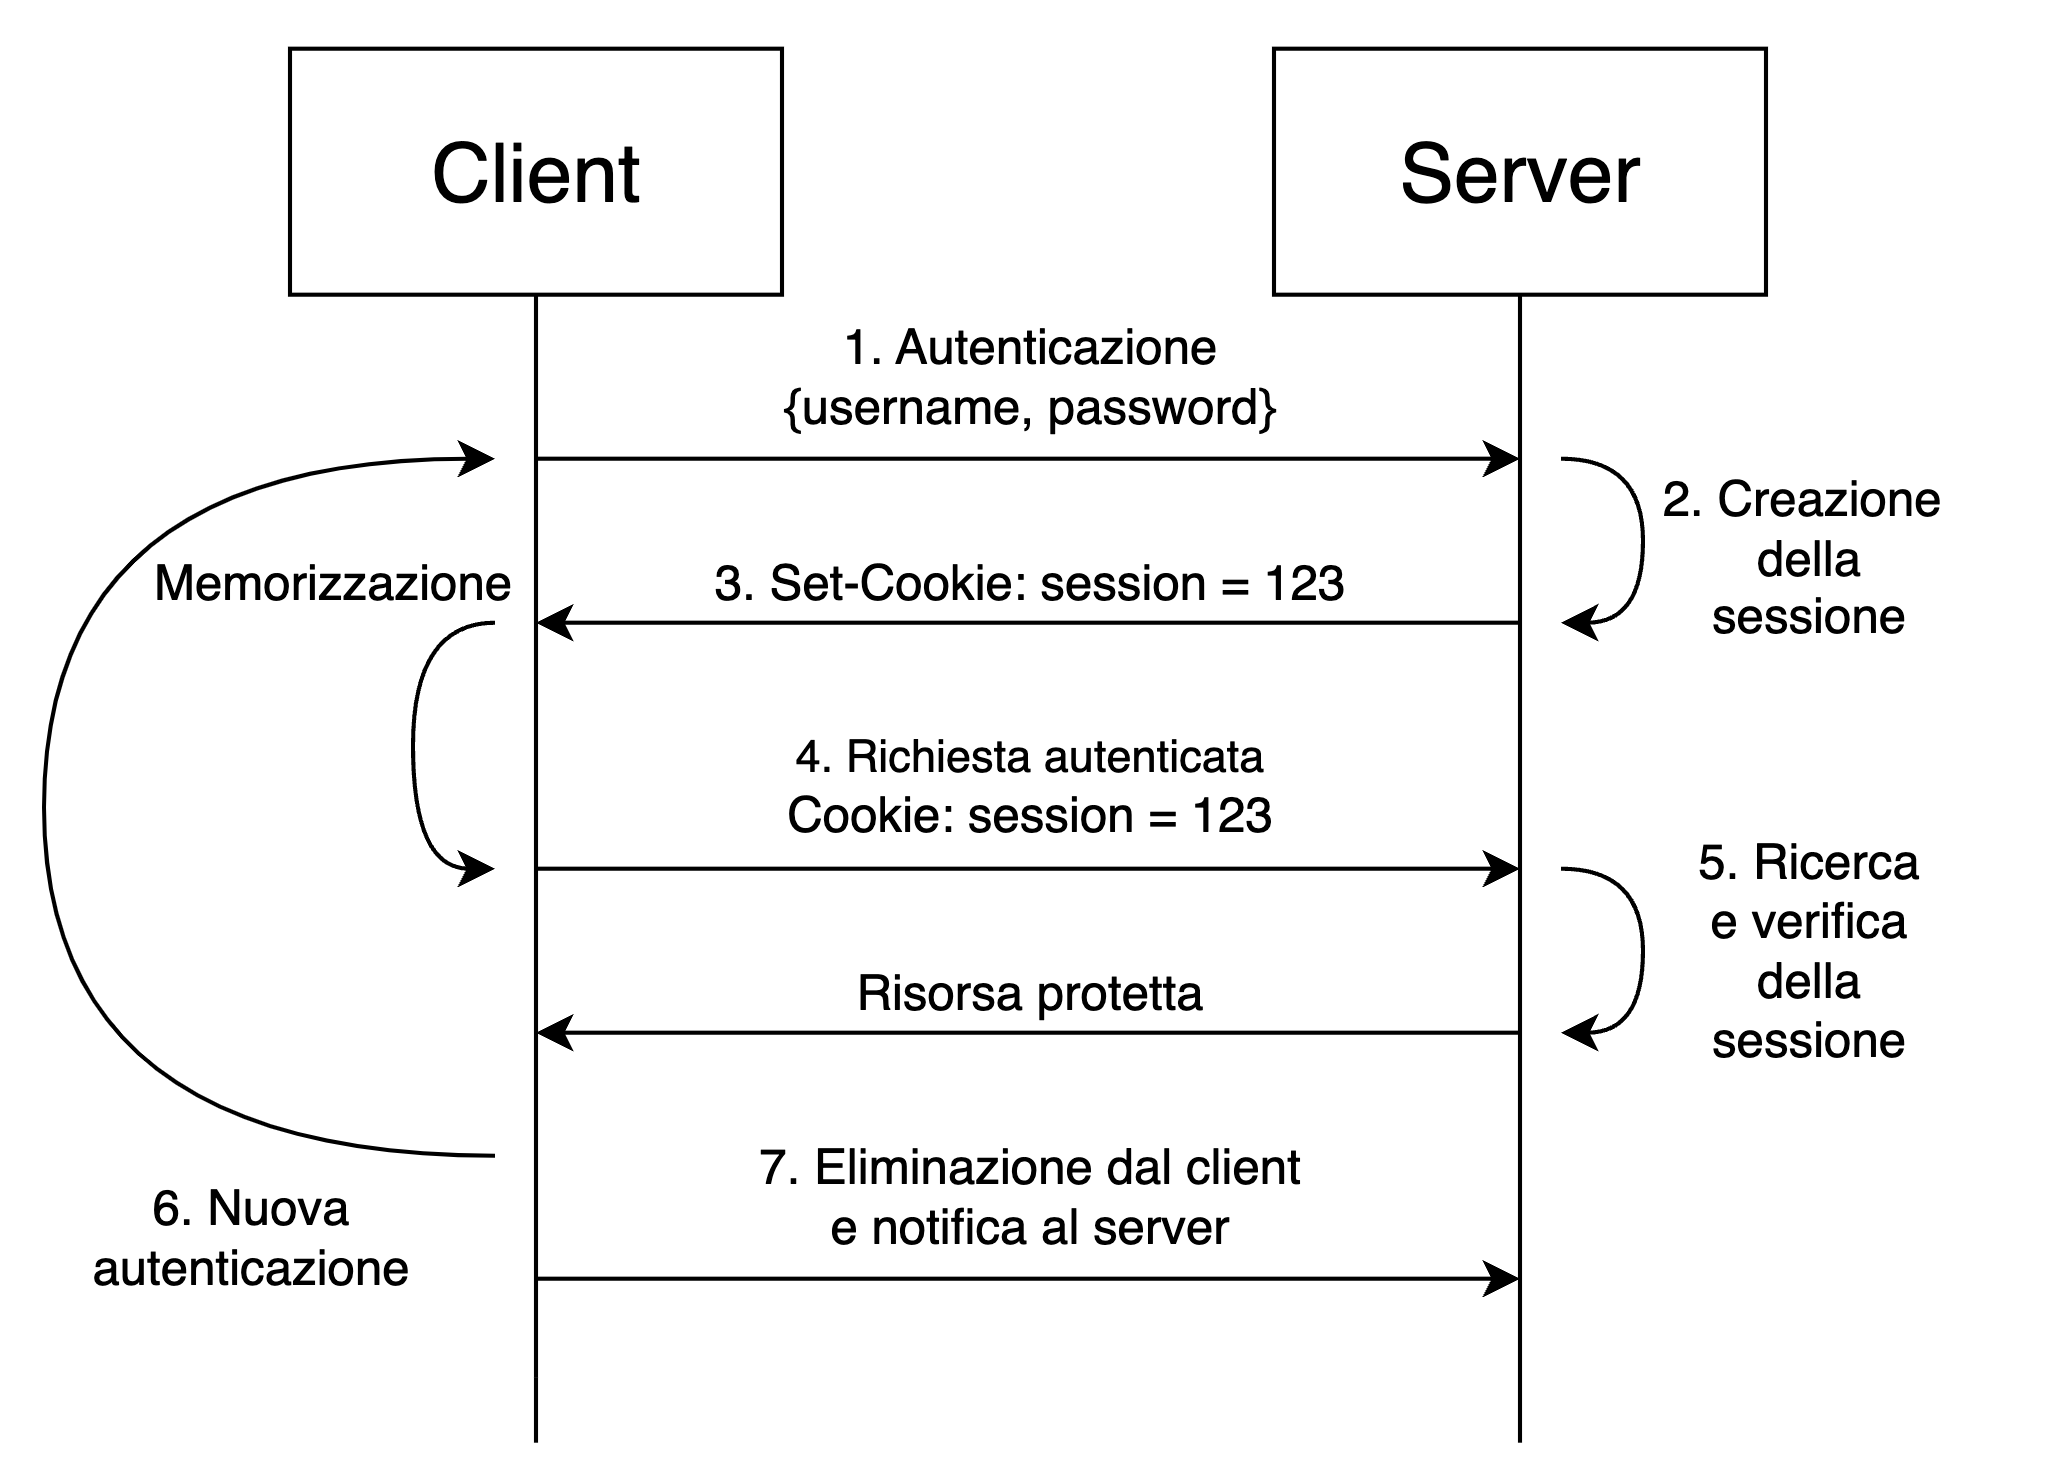
\includegraphics[width=0.9\columnwidth]{descrizione-stage/auth-cookie-based} 
    \caption{Processo di autenticazione basato su cookie}
	\label{fig:auth-cookie-based}
\end{figure}

\noindent L'utilizzo di cookie per l'autenticazione ha molti vantaggi.
Il principale è che sono supportati da tutti i browser e sono facili da implementare, in quanto è il browser stesso a gestirne la memorizzazione e l'invio.
I cookie inoltre necessitano di poca memoria e possono essere utilizzati anche per i \emph{sottodomini} di un sito web.

Tuttavia, l'autenticazione basata su cookie ha anche dei limiti.
Infatti, essi sono vulnerabili ad attacchi di tipo \emph{Cross-Site Scripting (XSS)} e \emph{Cross-Site Request Forgery (CSRF)} e non sono adatti per le architetture senza stato (dall'inglese \emph{stateless}), come alcuni tipi di \emph{\gls{API}}\glsfirstoccur.
Inoltre, i cookie non sono facilmente scalabili e non sono adatti per le applicazioni distribuite, in quanto dovrebbero essere memorizzati in un \emph{database} condiviso che potrebbe aumentare la complessità dell'applicazione.

\subsection{Autenticazione basata su token}
Un metodo di autenticazione alternativo all'utilizzo dei cookie è l'autenticazione basata su token.
Questo metodo è diventato molto popolare negli ultimi anni grazie all'aumento delle applicazioni web single page, al maggiore utilizzo di \emph{\gls{API RESTful}}\glsfirstoccur e dalla diffusione di dispositivi \emph{\gls{IoT}}\glsfirstoccur.

Un token è un oggetto simbolico rilasciato da un'autorità fidata\footcite{site:token-based-authentication-cloudflare}, ovvero il server, che permette all'utente di accedere a una risorsa protetta.
Diversamente dai cookie, i token sono \emph{stateless}, dunque non è necessaria la memorizzazione di alcuna informazione sul server.
Ciò è possibile perché ogni token contiene tutte le informazioni necessarie per la verifica dell'identità dell'utente e per l'accesso alla risorsa protetta. \\

\noindent Analogamente ai cookie, l'autenticazione basata su token viene effettuata nel seguente modo, come illustrato in figura \ref{fig:auth-token-based}:
\begin{enumerate}
	\item L'utente che vuole accedere alla risorsa protetta inserisce le proprie credenziali.
	\item Il server verifica le credenziali e, se corrette, genera un token con tutte le informazioni necessarie per l'accesso alla risorsa protetta.
	\item Il token viene inviato al client, il quale lo memorizza in modo sicuro.
	\item A questo punto, quando il client ha bisogno di accedere a una risorsa prottetta, include il token nella richiesta.
	\item Il server verifica la sua validità e consente l'accesso alla risorsa richiesta. 
	\item In caso di scadenza, l'utente deve autenticarsi nuovamente per ottenere un nuovo token.
	\item Quando viene effettuato il logout, il token viene cancellato dal client. Il server, invece, essendo senza stato, non ha bisogno di effettuare ulteriori operazioni.
\end{enumerate}

\begin{figure}[!ht] 
	\centering 
	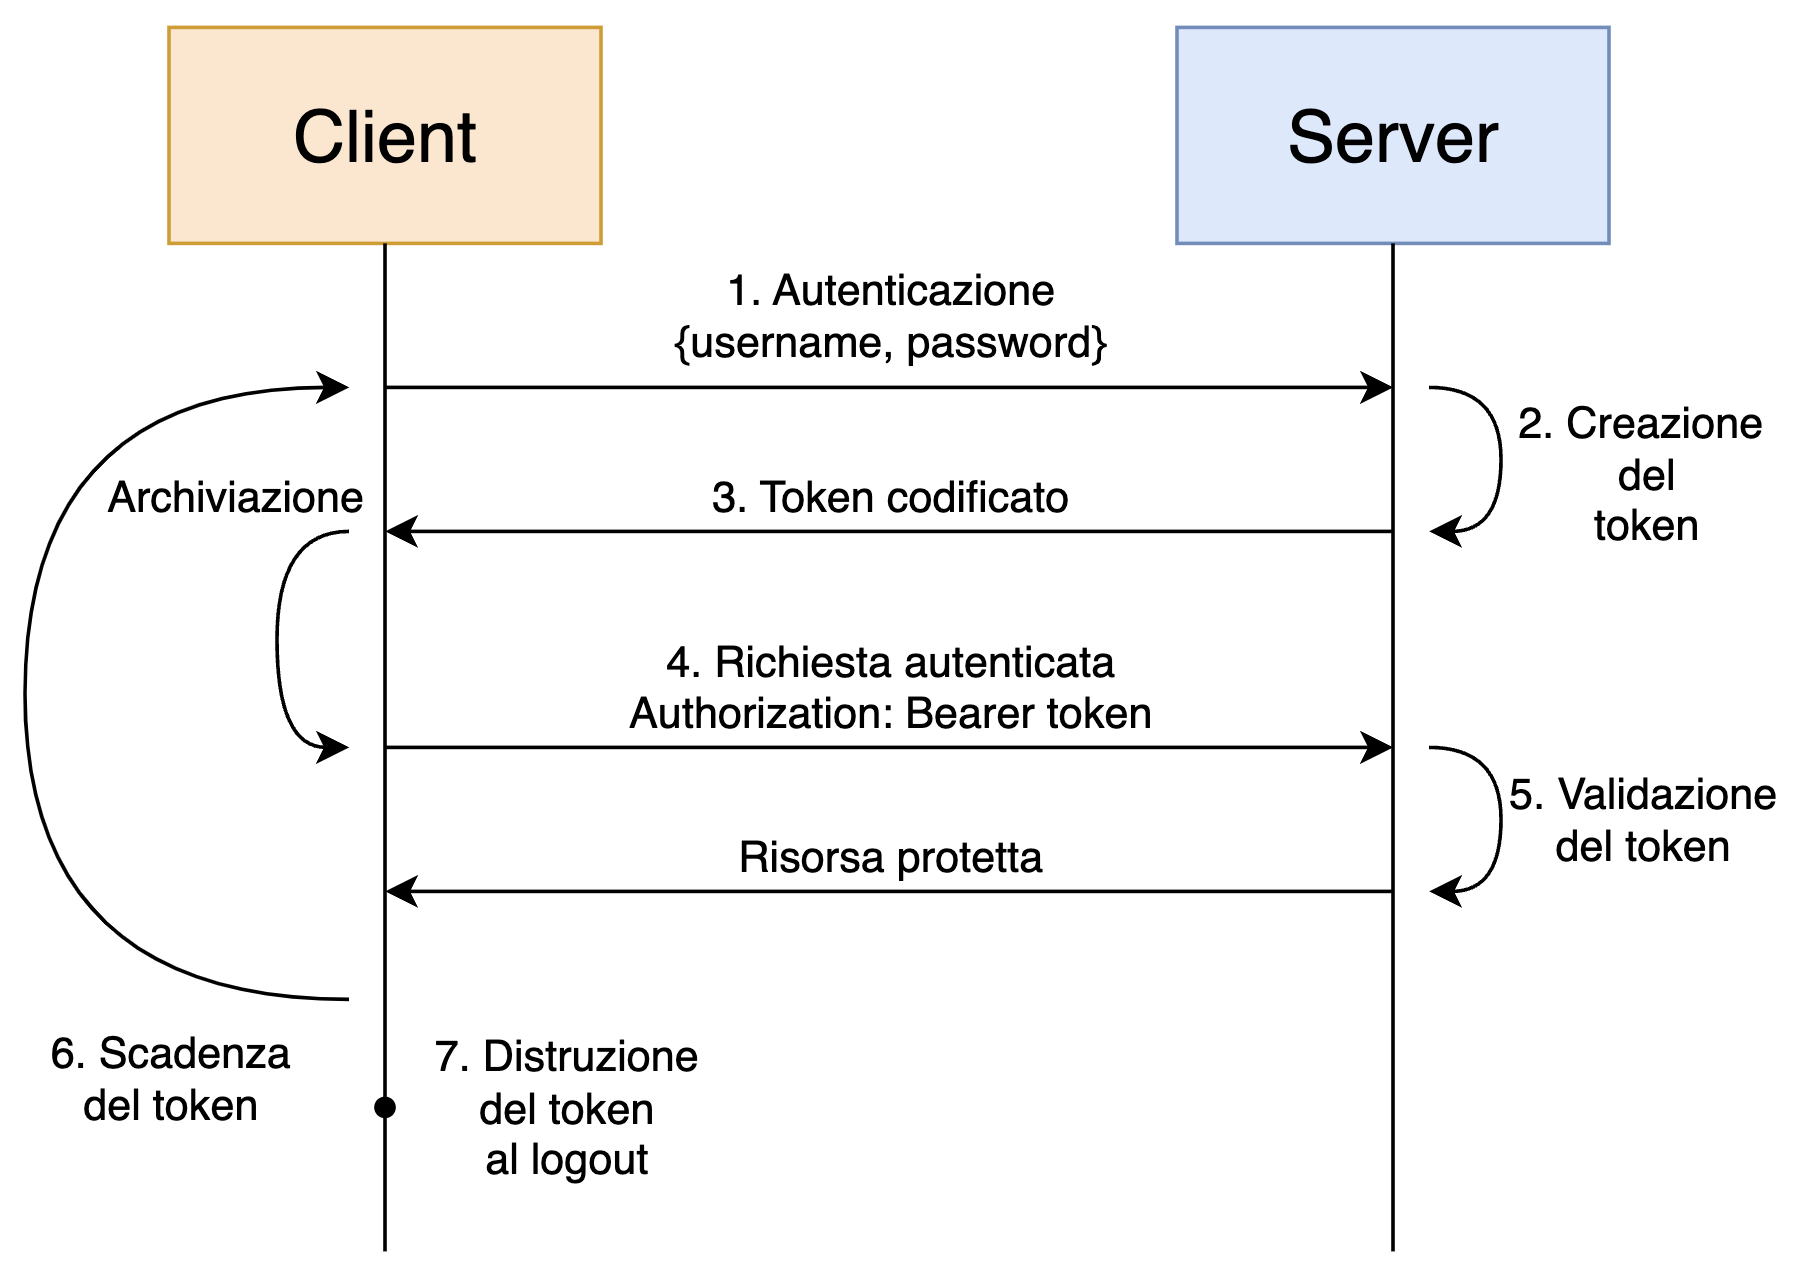
\includegraphics[width=0.9\columnwidth]{descrizione-stage/auth-token-based} 
	\caption{Processo di autenticazione basato su token}
	\label{fig:auth-token-based}
\end{figure}

\noindent L'utilizzo di questo metodo di autenticazione permette, dal lato server, di velocizzarne il processo, poiché non è necessaria nessuna verifica nel database.
Inoltre, la presenza di dati addizionali all'interno del token, come il livello dei permessi dell'utente, consente di semplificare ulteriormente il processo.
D'altro canto, questi campi addizionali aumentano notevolmente le dimensioni, rendendo la trasmissione e l'archiviazione più onerose.

Tuttavia, il più grande vantaggio dell'autenticazione basata su token è la possibilità di essere utilizzata anche per applicazioni mobili e \emph{API} che non si interfacciano con un browser.
I cookie, infatti, non si interfacciano correttamente con applicazioni native per dispositivi mobili, mentre i token possono essere facilmente integrati in qualsiasi applicazione con le stesse \emph{API}, se scritti correttamente.
In aggiunta, sono anche facilmente implementabili in applicazioni distribuite, come quelle per dispositivi \emph{IoT}.\\

\noindent Questo documento si concentra sull'autenticazione basata su token, in particolare su quelli di tipo \emph{JSON Web Token (JWT)}.


\section{Introduzione all'implementazione}
Uno dei vantaggi dell'utilizzo di metodi \emph{stateless} è la possibilità di integrarli facilmente in qualsiasi applicazione, indipendentemente dalla tecnologia utilizzata.
L'impossibilità di utilizzare i cookie senza l'ausilio di un browser rende i token la scelta migliore per applicazioni che utilizzano \emph{API RESTful}.

Per completare questo studio, è stato richiesto di implementare un \emph{ChatBot} in \emph{C\#} per la piattaforma di messaggistica Microsoft Teams utilizzando le \emph{API} di Microsoft Graph e token firmati e crittografati per garantire la sicurezza e la riservatezza di tutti i dati scambiati.

\subsection{Microsoft Teams}

\begin{figure}[!ht] 
	\centering 
	
\includegraphics[width=0.3\columnwidth]{descrizione-stage/logo-teams} 
	\caption{Logo di Microsoft Teams}
\end{figure}

Microsoft Teams\footcite{site:microsoft-teams} è una piattaforma di messaggistica e collaborazione offerta da Microsoft.
Essa consente a organizzazioni, team e singoli utenti di comunicare e collaborare con colleghi e clienti in tempo reale tramite chat, videoconferenze e chiamate.
Il \emph{ChatBot} implementato su questa piattaforma consentirà ai clienti di Prorob S.r.l di interagire con i servizi di Quindi Production Copilot in un modo più semplice e veloce.

\subsection{Microsoft Graph}

\begin{figure}[!ht] 
	\centering 
	
\includegraphics[width=0.3\columnwidth]{descrizione-stage/logo-graph} 
	\caption{Logo di Microsoft Graph}
\end{figure}

Microsoft Graph\footcite{site:microsoft-graph} è una piattaforma di sviluppo che unifica le \emph{API} di Microsoft 365 e Azure, permettendo alle applicazioni sviluppate da terze parti di interagire con i dati memorizzati nei vari servizi di Microsoft.
Utilizzando le \emph{API} di Microsoft Graph, il \emph{ChatBot} può interagire con con la chat di Teams, inviando messaggi e ricevendo notifiche.

\section{Obiettivi}
Prima dell'inizio dello stage Prorob S.r.l ha definito un piano di lavoro con gli obiettivi da raggiungere durante le 300-320 ore di stage. \\

\noindent Gli obiettivi principali prevedevano:
\begin{itemize}
	\item Studio dei \emph{JSON Web Token} e dei loro metodi di firma e di crittografia.
	\item Implementazione di una tecnologia generatrice di token \emph{API} firmati con certificati creati da chiavi ellittiche ed autenticati con metodologia \emph{HMAC}.
	\item Contribuire attivamente all'organizzazione e all'avanzamento delle attività in team.
\end{itemize}

Tuttavia, durante le settimane di stage, gli obiettivi iniziali sono stati rivisti in base alle esigenze emerse. Questo ha portato alla rimozione del un obiettivo e alla definizione di uno nuovo.
Infatti è stata rimossa l'implementazione della tecnologia generatrice di token \emph{API} firmati ed è stata sostituita con l'implementazione di un \emph{ChatBot} per la piattaforma di Microsoft Teams utilizzando i \emph{JWT} e algorithmi di firma e crittografia. \\

\noindent Gli obiettivi finali, dunque, sono stati:
\begin{itemize}
	\item Studio dei \emph{JSON Web Token} e dei loro metodi di firma e di crittografia.
	\item Implementazione di un \emph{ChatBot} per la piattaforma di messaggistica Microsoft Teams utilizzando i \emph{JWT} e algoritmi di firma e crittografia.
	\item Contribuire attivamente all'organizzazione e all'avanzamento delle attività in team.
\end{itemize}
    \chapter{Autenticazione con JSON Web Token}
\label{cap:autenticazione-jwt}

% \intro{Breve introduzione al capitolo}\\

\section{Cosa è un JSON Web Token?}

\emph{JSON Web Token (JWT)} è uno standard aperto (\emph{RFC 7519}\footcite{site:rfc7519}) che definisce un modo compatto per trasmettere informazioni in modo sicuro tra due parti come oggetti \emph{\gls{JSON}}.
Queste informazioni possono essere verificate e attendibili perché sono firmate digitalmente.

Le firme digitali possono essere generate utilizzando algoritmi \emph{\gls{HMAC}} (chiave segreta), \emph{\gls{RSA}} (coppia chiave pubblica/privata) o \emph{\gls{ECC}} (curve ellittiche).

\noindent I \emph{JWT} vengono utilizzati principalmente per:
\begin{itemize}
	\item \textbf{Autenticazione}: Una volta che un utente si è autenticato, il server può generare un \emph{JWT}, che può essere utilizzato per accedere a risorse specifiche senza dover autenticare l'utente ogni volta.
	      Questo è utile per le \emph{API RESTful}, dove l'autenticazione è necessaria per ogni richiesta.
	      \emph{\gls{SSO}} è un altro esempio di utilizzo per l'autorizzazione.
	\item \textbf{Scambio di informazioni}: Poiché i \emph{JWT} possono essere firmati, si può essere sicuri che il mittente sia chi dice di essere e che i contenuti del messaggio non siano stati alterati.
\end{itemize}

\subsection{Struttura di un JWT}
Un \emph{JWT} è composto da tre parti separate da punti: \emph{header}, \emph{payload} e \emph{signature}.
La struttura generale è come segue:

$$header.payload.signature$$

L'\emph{header} (intestazione) contiene il tipo di algoritmo di firma utilizzato e il tipo di token.
Questo \emph{JSON} viene poi codificato in \emph{Base64URL}, una codifica \emph{\gls{Base64}} sicura per gli \emph{\gls{URL}}.

\noindent Un esempio di \emph{header} in formato \emph{JSON} è il seguente:
\begin{verbatim}
{
	"alg": "HS256",
	"typ": "JWT"
}
\end{verbatim}

Il \emph{payload} (contenuto) contiene le informazioni che si desidera trasmettere, generalmente riguardanti un'entità (solitamente l'utente) e/o metadati.
Queste informazioni, come anche quelle contenute nell'\emph{header}, vengono rappresentate sotto forma di coppie chiave-valore chiamate \emph{claim}.
È importante notare che il \emph{payload} non è crittografato, quindi non dovrebbe contenere informazioni sensibili se il token non viene inviato su una rete sicura.
Anche il \emph{payload JSON} viene codificato in \emph{Base64URL}.

\noindent Un esempio di \emph{payload} è il seguente:
\begin{verbatim}
{
	"sub": "1234567890",
	"name": "Nicolò Pellegrinelli",
	"admin": true
}
\end{verbatim}

La \emph{signature} (firma) viene generata combinando le prime due parti con una chiave segreta.
L'algoritmo di firma specificato nell'\emph{header} determina il metodo esatto utilizzato per calcolare la firma.
La \emph{firma} è un passaggio critico per garantire l'integrità del token.
Essa consente di verificare che il contenuto del token non sia stato alterato durante la trasmissione o la memorizzazione.
Questo è fondamentale in scenari dove la sicurezza e l'affidabilità delle informazioni sono cruciali, come nell'autenticazione e nell'autorizzazione di utenti.

In aggiunta alla protezione dell'integrità, se il token è stato firmato utilizzando una chiave privata, la firma può essere anche utilizzata per autenticare l'identità del mittente.
Questo processo assicura che il token sia stato emesso da una fonte attendibile e autorizzata, rafforzando ulteriormente la sicurezza del sistema.\\

Utilizzando la chiave segreta $lrdoyfMvYppQTQC2O0AGVanBCsThRhmV$ il token \emph{JWT} risultante dall'esempphio precedente risulterebbe come segue: \\


\noindent \emph{\textcolor{blue}{eyJhbGciOiJIUzI1NiIsInR5cCI6IkpXVCJ9}}.

\noindent \emph{\textcolor{red}{eyJzdWIiOiIxMjM0NTY3ODkwIiwibmFtZSI6Ik5pY29sw7IgUGVsbGVncmluZWxsaSIs}}
\noindent \emph{\textcolor{red}{ImFkbWluIjp0cnVlfQ}}.

\noindent \emph{\textcolor{olive}{ILwwP\_3ZNcV-wf0VMYsD1HFm8CM2GLg-aVDZdvBmI7I}}\\

L'esempio appena mostrato può essere decodificato utilizzando lo strumento online \cite{site:jwt-debugger}.


\subsection{Funzionamento di un JWT}
Quando un utente si autentica, un token \emph{JWT} viene generato e inviato al client.
Ogni volta che l'utente farà una richiesta al server, questo token verrà inviato con la richiesta.
A questo punto il server può verificare la firma del token per assicurarsi che sia valido e che l'utente abbia i permessi necessari per accedere alla risorsa richiesta.

Generalmente i \emph{JWT} hanno una scadenza breve per garantire un livello di sicurezza alto.
Questi token sono chiamati \emph{Access Token}\footcite{site:rfc6749} e sono quelli utilizzati per l'accesso alle risorse protette.
Un altro tipo di token è il \emph{Refresh Token}, che viene utilizzato per ottenere un nuovo \emph{Access Token} una volta che il precedente è scaduto.
I \emph{Refresh Token} hanno una vita più lunga degli \emph{Access Token} e interagiscono con gli \emph{authorization server} invece dei \emph{resource server}\footnote{L'\emph{authorization server} è il server che rilascia i token, mentre il \emph{resource server} è il server che contiene le risorse protette.}.

\noindent Questo procedimento viene illustrato in figura \ref{fig:jwt-flow}.

\begin{figure}[!ht] 
    \centering 
    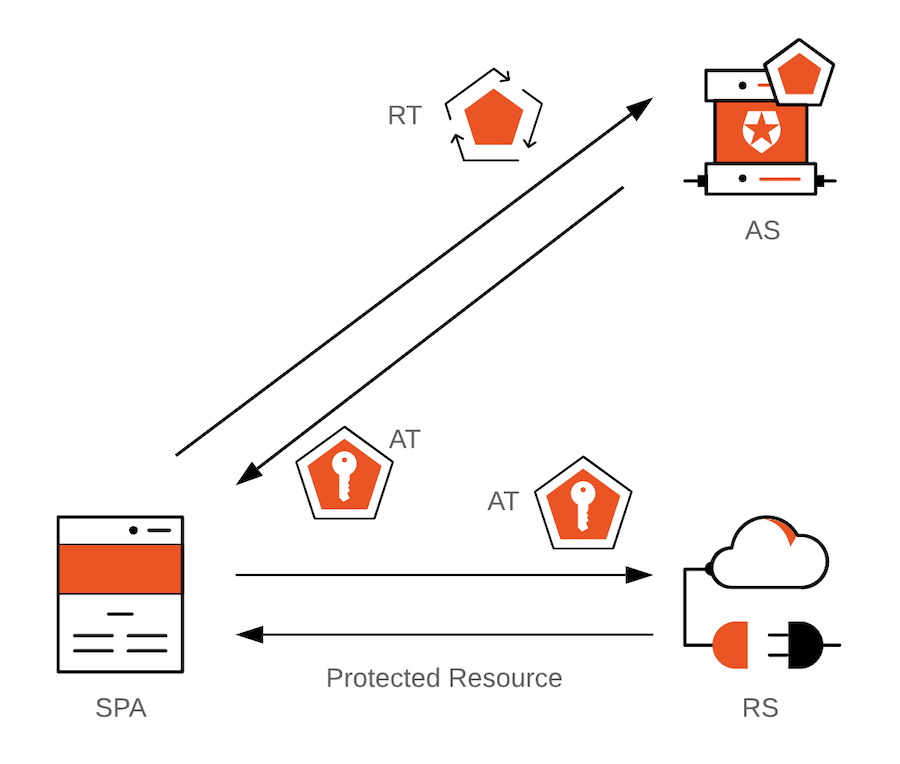
\includegraphics[width=0.7\columnwidth]{autenticazione/rt-and-at} 
    \caption{Flusso dei token JWT. RT = Refresh Token; AT = Access Token; AS = Authorization Server (Server di Autorizzazione); RS = Resourse Server (Server di Risorsa); SPA = Single Page Application (Applicazione Web). Fonte: \cite{site:jwt-flow}}
	\label{fig:jwt-flow}
\end{figure}

\section{Standard di sicurezza per JWT}
I \emph{JWT} sono uno standard aperto e flessibile, il che significa che possono essere utilizzati in molti contesti diversi.
Tuttavia, per garantire la sicurezza dei token e dei dati che contengono, è importante seguire alcune \emph{best practices}\footnote{Le best practices (migliori pratiche) sono linee guida raccomandate per ottenere risultati ottimali. Seguendo queste linee guida, si possono evitare errori comuni e migliorare efficienza, qualità e sicurezza di processi e prodotti.} e standard di sicurezza.

\subsection{JSON Web Encryption}
Il \emph{\gls{JWE}} standard stabilisce un modo per crittografare, e quindi rendere oscuri, i contenuti di un \emph{JWT}.
A primo impatto, potrebbe sembrare che la crittografia abbia le stesse garanzie della firma, con l'aggiunta della riservatezza dei dati.
Tuttavia la crittografia non garantisce l'autenticità dei dati, ma solo la loro riservatezza.

Il \emph{JWE} supporta principalmente due schemi: uno schema a chiave segreta e uno a chiave pubblica.
Lo schema a chiave segreta funziona in modo che ogni parte che detiene la chiave segreta può crittografare e decrittografare i dati

Lo schema a chiave pubblica, invece, funziona in maniera differente.
In questo caso sono le parti che detengono la chiave pubblica a crittografare i dati, mentre la parte che detiene la chiave privata può decrittografarli.
In pratica, chi detiene la chiave pubblica può creare nuovi messaggi crittografati.
Questo, però, non vuol dire che chi crittografa i dati è sempre chi sostiene di essere. Di conseguenza, la crittografia non può fornire le stesse garanzie di autenticità come per la firma.

Per questi motivi \emph{JWE} è spesso utilizzato in combinazione con \emph{\gls{JWS}}: un token crittografato funziona da container per un token firmato in modo da ottere i benefici di entrambi.

\subsection{JSON Web Signature}
Il \emph{JSON Web Signature (JWS)} stabilisce un singolo algoritmo di firma supportato da tutte le implementazioni: \emph{\hyperref[sec:hmac]{HMAC}} con \emph{\gls{SHA-256}}, chiamato \emph{HS256}.
Tuttavia, secondo il \emph{\gls{JWA}} standard, anche altri algoritmi sono consigliati per l'uso con \emph{JWT}.
Tra questi \emph{\hyperref[sec:rsassa]{RSASSA PKCS1 v1.5}} con \emph{SHA-256 (RS256)} e \emph{\hyperref[sec:ecdsa]{ECDSA}} con \emph{\gls{P-256}} a curva ellittica e \emph{SHA-256 (ES256)}\footnote{Questi algoritmi vengono descritti nei paragrafi successivi}.


\section{HMAC}
\label{sec:hmac}

\emph{Keyed-Hash Message Authentication Code (HMAC)} è un algoritmo di firma che combina un certo messaggio con una chiave segreta utilizzando una funzione \emph{hash} crittografica.
Il risultato è un codice di autenticazione che può essere utilizzato per verificare un messaggio solo se le parti generatrice e verificatrice condividono la stessa chiave segreta.

La robustezza della funzione \emph{hash} garantisce che il messaggio non possa essere modificato senza conoscere la chiave segreta.

In sostanza, \emph{HMAC} permette di verificare l'integrità e l'autenticità di un messaggio attraverso chiavi segrete condivise.

\noindent Sia:
\begin{itemize}
	\item $H$ la funzione \emph{hash} crittografica
	\item $B$ la lunghezza del blocco di $H$
	\item $K$ la chiave segreta
	\item $K'$ la vera chiave utilizzata da $H$ e derivata da $K$
	\item $ipad$ il byte \emph{0x36} ripetuto $B$ volte (chiamato anche padding interno)
	\item $opad$ il byte \emph{0x5C} ripetuto $B$ volte (chiamato anche padding esterno)
	\item $M$ il messaggio
	\item $||$ l'operatore di concatenazione
\end{itemize}

\noindent L'algoritmo \emph{HMAC} è definito come:
% \begin{verbatim}
\begin{equation}
	\begin{aligned}
		&HMAC(K, M) = H((K' \oplus opad) || H((K' \oplus ipad) || M))
	\end{aligned}
\end{equation}

\noindent dove $\oplus$ è l'operatore di \emph{XOR}\footnote{Lo XOR (o OR esclusivo) è un'operazione binaria che restituisce 1 se e solo se uno degli operandi è 1, altrimenti restituisce 0} e $K'$ è definito come segue:
\begin{itemize}
	\item Se $K$ è più corto di $B$, vengono aggiunti zeri a sinistra per raggiungere la lunghezza di $B$.
	\item Se $K$ è più lungo di $B$, viene calcolato $H(K)$.
	\item Se $K$ è esattamente di $B$ byte, $K'$ è uguale a $K$.
\end{itemize}

\noindent La funzione \emph{HS256} è un esempio di algoritmo \emph{HMAC} che utilizza la funzione di \emph{hash} \emph{SHA-256}.


\section{RSA}
Gli algoritmi a chiave pubblica si basano sulla generazione di due chiavi, una privata e una pubblica, per crittografare e decrittografare rispettivamente i dati.

L'algoritmo \emph{RSA}, uno dei più noti algoritmi a chiave pubblica, si fonda sulla complessità del problema della fattorizzazione dei numeri interi composti.
La sicurezza di \emph{RSA} deriva dal fatto che, mentre è relativamente facile moltiplicare due numeri primi per ottenere un numero composto, è estremamente difficile eseguire l'operazione inversa, ossia fattorizzare un numero composto per ottenere i due numeri primi originali.

\noindent Questo problema può essere rappresentato come segue:
\begin{equation}
	\begin{aligned}
		&(m^e)^d \equiv m \mod n
	\end{aligned}
\end{equation}

\noindent $m$ è il messaggio originale ed $e$, $d$ e $n$ sono scelti nel seguente modo:
\begin{enumerate}
	\item $p$ e $q$ sono due grandi primi generati casualmente.
	      \begin{itemize}
		      \item Un \emph{\gls{RNG}} crittograficamente sicuro dovrebbe essere utilizzato per generare questi numeri.
		      \item Non esistendo modo di generare randomicamente numeri primi, è necessario verificare che i numeri generati siano effettivamente primi.
		      \item I numeri primi devono essere grandi e simili per ordine di grandezza.
	      \end{itemize}
	\item $n$ è il risultato del prodotto $p \cdot q$. Questo numero è il modulo e il suo numero di bit equivale alla lunghezza della chiave.
	\item $\phi(n) = (p - 1) \cdot (q - 1)$ è il quoziente di Eulero ($phi(n)$).
	\item $e$ è un numero intero scelto in modo che $1 < e < \phi(n)$ e $e$ sia coprimo con $\phi(n)$.
	\item $d$ deve soddisfare la congruenza $d \equiv e^{-1} \mod \phi(n)$.
	      \begin{itemize}
		      \item $d$ è l'inverso moltiplicativo di $e$ modulo $\phi(n)$.
		      \item L'equazione può essere riscritta come $e \cdot d \equiv 1 \mod \phi(n)$.
	      \end{itemize}
\end{enumerate}

La chiave pubblica è composta dai valori di $n$ ed $e$, mentre la chiave privata è composta dai valori di $n$ e $d$.

$p$, $q$ e $\phi(n)$ sono valori che devono essere mantenuti segreti.

Questa proprietà consente a chiunque abbia la chiave pubblica di crittografare un messaggio, ma solo chi possiede la chiave privata sarà in grado di decrittografarlo.

\subsection{Firma e Verifica con RSA}
\label{sec:rsassa}

L'algoritmo \emph{RSA} non è solo utilizzato per la crittografia, ma anche per la firma digitale.
La caratteristica principale dell'avere una coppia di chiavi pubblica e privata permette di utilizzare \emph{RSA} per creare firme digitali che permettono a chiunque di verificare l'origine e l'integrità del messaggio firmato utilizzando la chiave pubblica.
Infatti, solamente chi è in possesso della chiave privata può creare la firma.
Le chiavi pubbliche invece possono essere distribuite liberamente poichè non permettono di creare nuove firme, ma solo di validarle.

\noindent Il processo di firma e verifica funziona come segue:
\begin{enumerate}
	\item Un \emph{digest}\footnote{Un \emph{digest} è un breve valore risultato da un blocco di dati più grande tramite una funzione \emph{hash}. Funziona come una "impronta digitale" dei dati, permettendo di verificare l'integrità e l'autenticità dei dati stessi senza bisogno di conoscere l'intero contenuto originale.} del messaggio viene calcolato da una funzione hash.
	\item Il \emph{digest} viene poi elevato alla potenza di $d$ modulo $n$ (chiave privata).
	\item Il risultato è aggiunto al messaggio come firma.
\end{enumerate}
\noindent Per verificare la firma invece:
\begin{enumerate}
	\item La firma viene elevata alla potenza di $e$ modulo $n$ (chiave pubblica). Questo restituisce il \emph{digest} originale.
	\item Viene calcolato il \emph{digest} del messaggio ricevuto, utilizzando la stessa funzione \emph{hash} del passaggio di firma.
	\item Se i due \emph{digest} sono uguali, la firma è valida.
\end{enumerate}

Questo processo è conosciuto come \emph{\gls{SSA}}, infatti la firma è un "appendice" del messaggio originale in quanto è necessario nel processo di verifica della firma.
Questo schema permette dunque la possibilità di distribuire in modo sicuro uno-a-molti messaggi firmati: le parti riceventi possono verificare l'autenticità del messaggio mantenendo una copia della chiave pubblica, ma non possono creare nuovi messaggi con essa.

\emph{RSASSA} è una famiglia di schemi di firme digitali basati su \emph{RSA} che utilizzano \emph{SSA}.
Tra questi algoritmi possiamo trovare \emph{RSASSA-PKCS1-v1\_5} che utilizza un tipo di padding specifico descritto nello standard \emph{\gls{PKCS1} v1.5}.
L'utilizzo della funzione di \emph{hash SHA-256} permette di rendere la firma di \emph{RS256}\footnote{RSASSA-PKCS1-v1\_5 con SHA-256} crittograficamente sicura.

\section{ECC}
L'esistenza di algoritmi di fattorizzazione efficienti come il \emph{\gls{GNFS}} o il \emph{\gls{QS}} ha reso \emph{RSA} con chiavi brevi vulnerabile.
Questo ha portato alla necessità di utilizzare chiavi sempre più lunghe per garantire un livello di sicurezza accettabile.
Tuttavia, con l'aumentare della lunghezza delle chiavi, anche il tempo di calcolo per le operazioni \emph{RSA} aumenta significativamente.
Questo compromesso tra sicurezza e performance diventa insostenibile sul lungo periodo, in particolare per dispositivi con risorse limitate.
Ciò può potenzialmente rendere \emph{RSA} insicuro e non più utilizzabile.

L'\emph{ECC} consente di creare algoritmi crittografici più efficienti.
Tra questi, l'\emph{\hyperref[sec:ecdh]{Elliptic Curve Diffie-Hellman (ECDH)}} per lo scambio di chiavi e l'\emph{Elliptic Curve Digital Signature Algorithm (ECDSA)} per la firma digitale sono i più comuni.
Anche questo tipo di algoritmi genera una coppia di chiavi privata/pubblica, ma utilizza, invece della fattorizzazione di numeri semiprimi, il logaritmo discreto su curve ellittiche.

\noindent Le curve ellittiche per la crittografia sono definite dalla seguente equazione di terzo grado:

\begin{equation}
	\begin{aligned}
		&y^2 = x^3 + ax + b
	\end{aligned}
\end{equation}

\noindent dove $a$ e $b$ sono parametri della curva.

Gli algoritmi a curve ellittiche sono definiti su campi primi finiti, ovvero insiemi di numeri interi su cui sono definite due operazioni binarie: somma e moltiplicazione.
Con campo primo finito si intende che il numero di elementi nel campo è un numero primo $p$, quindi una quantità finita. Tutti gli elementi e le operazioni sono definite modulo $p$.

Rendendo il campo finito, gli algoritmi usati per le operazioni matematiche cambiano.
In particolare, il logaritmo discreto viene usato al posto del logaritmo normale.

Essendo il campo composto da un numero finito di elementi, si potrebbe pensare che il logaritmo discreto diventi un problema semplice, tuttavia, non esiste ad oggi un algoritmo efficiente per la risoluzione del logaritmo discreto su curve ellittiche.
Questa proprietà rende il logaritmo discreto ideale per la crittografia e la firma digitale.

Per rendere però l'algoritmo sicuro, è necessario che la curva, ovvero i parametri $a$ e $b$, sia scelta in modo corretto. In passato, infatti, si sono verificati casi in cui certi parametri hanno reso le curve deboli.

\noindent Un esempio di curva ellittica è illustrato in figura \ref{fig:curva-ellittica}. L'equazione della curva è la seguente:

\begin{equation}
	\begin{aligned}
		&y^2 = x^3 - 3x + 25
	\end{aligned}
\end{equation}


\begin{figure}[!ht] 
    \centering 
    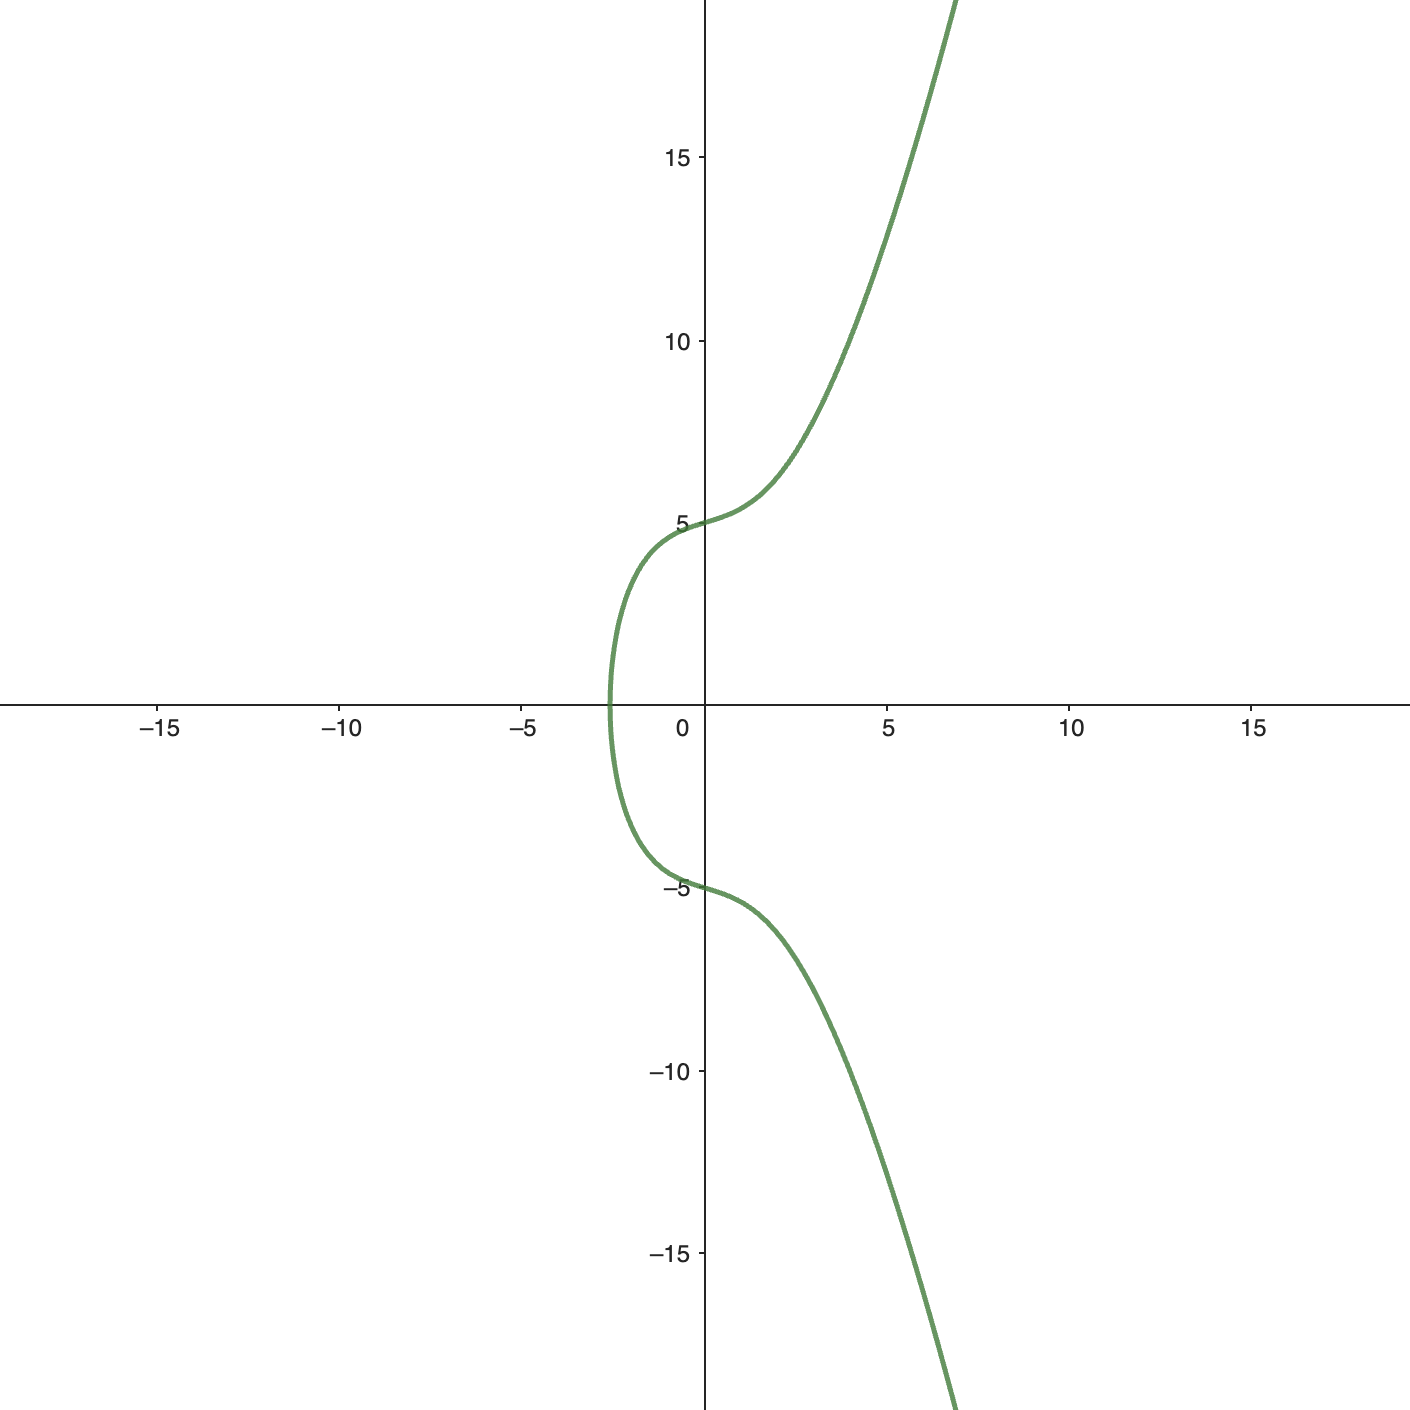
\includegraphics[width=0.7\columnwidth]{autenticazione/curva-ellittica} 
    \caption{Grafico di una curva ellittica}
	\label{fig:curva-ellittica}
\end{figure}

L'aspetto interessante degli algoritmi a curva ellittica è che la lunghezza della chiave può essere ridotta di molto rispetto a \emph{RSA} per ottenere lo stesso livello di sicurezza.
Per esempio, una chiave EC\footnote{Chiave generata da una curva ellittica} di 256 bit è considerata sicura quanto una chiave \emph{RSA} di 3072 bit.

Ciò, oltre che a rendere più efficienti gli algoritmi, semplifica la trasmissione e la memorizzazione delle chiavi.
Il motivo per cui la chiave EC può essere più corta risiede nell'inesistenza, ad oggi, di algoritmi che risolvono il logaritmo discreto più efficientemente dell'approccio \emph{naive} o \emph{brute-force}\footnote{Con \emph{naive} o \emph{brute-force} si intende il "provare" tutti i valori possibili}, diversamente da \emph{RSA} che è più vulnerabile a fattorizzazione efficiente.

In un suo studio, il matematico Arjen K. Lenstra ha esposto il concetto di "Universal Security"\footcite{site:universal-security} calcolando l'energia necessaria per rompere determinti algoritmi crittografici e comparandola con la quantità di acqua che quell'energia sarebbe in grado di portare a ebollizione.
Con questo metodo, Lenstra ha dimostrato che per rompere una chiave \emph{RSA} di 228 bit è richiesta meno energia di quella necessaria per portare a ebollizione un cucchiaino d'acqua.
Al contrario, per rompere una chiave EC a 228 bit è necessaria una quantità di energia che porterebbe a ebollizione l'intera acqua presente sulla Terra.
Per questo livello di sicurezza con \emph{RSA} è necessaria una chiave di almeno 2380 bit.

\subsection{Usi di ECC}
Nonostante la sua sicurezza e la sua efficienza, l'uso di \emph{ECC} è ancora limitato rispetto a \emph{RSA}.
Tuttavia, negli ultimi anni si è assistito ad un aumento nell'interesse per questa tecnologia e ad un incremento del suo utilizzo in varie applicazioni.
Il governo degli Stati Uniti, ad esempio, ha adottato \emph{ECC} per la crittografia delle comunicazioni, il progetto Tor lo utilizza per aiutare a garantire l'anonimato degli utenti e il protocollo \emph{\gls{TLS}} lo utilizza per garantire la sicurezza delle comunicazioni su Internet tramite \emph{\gls{HTTPS}}.
Anche i servizi di messaggistica di iMessage e Whatsapp utilizzano \emph{ECC} per garantire la sicurezza delle loro comunicazioni.
\emph{ECC} è inoltre utilizzato in molte applicazioni di blockchain, come Bitcoin ed Ethereum, al fine di approvare le transazioni.

\subsection{Elliptic Curve Digital Signature Algorithm (ECDSA)}
\label{sec:ecdsa}

L'\emph{Elliptic Curve Digital Signature Algorithm} è un algoritmo di firma digitale basato su curve ellittiche.
Il funzionamento è simile a quello di \emph{RSA}, ma utilizza curve ellittiche al posto dei numeri interi.

Immaginiamo che \emph{Utente A} voglia inviare un messaggio firmato a \emph{Utente B}.
\emph{A} sceglie in modo randomico un numero $d_A$ nel range $[1, n-1]$, che rappresenta la chiave private e dove $n$ è l'ordine del punto base $G$ della curva ellittica ed è un numero primo.
A questo punto, \emph{A} calcola il punto $Q_A = d_A \cdot G$\footnote{Nel contesto delle curve ellittiche indicheremo con il $\cdot$ del prodotto scalare la "moltiplicazione scalare delle curve ellittiche" (dall'inglese elliptic curve point multiplication). Questa è un'operazione che consiste nel sommare ripetutamente un punto $P$ sulla curva a se stesso un certo numero di volte $k$. La nomenclatura risulterà $P \cdot k$. \cite{site:ec-point-multiplication}} e la coordinata $x$ di $Q_A$. Il risultato è un punto della curva che rappresenta la chiave pubblica.
La curva ellittica e i suoi parametri (inclusi $G$ e $n$) vengono prestabiliti in base a uno standard crittografico.

\noindent Dunque, per firmare un messaggo \emph{Utente A} procede come segue:
\begin{enumerate}
	\item Calcola il digest $H(m)$ del messaggio $m$ con una funzione hash crittografica.
	\item $H(m)$ viene poi convertito in un numero intero intero $h$ ridotto modulo $n$.
	\item Un numero $k$ viene scelto randomicamente nel range $[1, n-1]$.
	\item Calcola il punto $k \cdot G$ e la sua coordinata $x$ viene ridotta modulo $n$, ottenendo $r$. Se $r = 0$, viene scelto un nuovo $k$.
	\item Calcola $s = (h + r \cdot d_A)/k \mod n$. Se $s = 0$, viene scelto un nuovo $k$.
	\item La coppia $(r, s)$ è la firma del messaggio.
\end{enumerate}

\noindent È importante notare che $k$ deve essere scelto in modo randomico e non deve essere mai riutilizzato con la stessa chiave privata.
L'utilizzo di $k$ più volte con la stessa chiave privata può portare alla compromissione della chiave privata.

\noindent Per verificare la firma \emph{Utente B} procede come segue:
\begin{enumerate}
	\item Verifica che $r$ e $s$ siano nel range $[1, n-1]$ e che $Q_A$ sia un punto sulla curva il cui prodotto con $n$ è l'elemento neutro.
	\item Calcola il digest $H(m)$ del messaggio $m$ con una funzione hash crittografica.
	\item $H(m)$ viene poi convertito in un numero intero intero $h$ ridotto modulo $n$.
	\item Calcola $w = s^{-1} \mod n$.
	\item Calcola $u_1 = hw \mod n$ e $u_2 = rw \mod n$.
	\item Calcola il punto $u_1 \cdot G + u_2 \cdot Q_A$ e la sua coordinata $x$ viene ridotta modulo $n$, ottenendo $v$.
	\item La firma è valida se $v = r$.
\end{enumerate}

\noindent \emph{ES256} è un esempio di algoritmo \emph{ECDSA} che utilizza la funzione di \emph{hash} \emph{SHA-256}.


\section{Diffie Hellman Key Exchange}
Il \emph{Diffie-Hellman Key Exchange (D-H)} è un protocollo crittografico che permette a due parti che non hanno una conoscenza pregressa di stabilire una chiave segreta condivisa su un canale di comunicazione non sicuro.
Questo protocollo fornisce le basi per una varietà di diversi protocolli crittografici. In particolare, è alla base della perfetta segretezza di \emph{TLS}, il protocollo utilizzato da \emph{HTTP(S)} per garantire la sicurezza delle comunicazioni.
Il protocollo originale, sviluppato da Whitfield Diffie e Martin Hellman nel 1976, non prevedeva la firma digitale e quindi non garantiva l'autenticità delle parti coinvolte nella comunicazione, rendendo il protocollo vulnerabile al \emph{\gls{MITM}}.

L'algoritmo si basa sulla difficoltà di calcolare il logaritmo discreto su campi finiti.
Inizialmente, le due parti scelgono un numero primo $p$ e un generatore $g$ del campo finito tale che $g^x \mod p$, per $x = 1, 2, ..., p-1$, generi tutti gli elementi del campo in qualche permutazione.
Per ogni intero $b$ minore di $p$ e radice primitiva di $p$, esiste un unico esponente $i$ tale che $b = a^i \mod p$. Questo esponente è chiamato logaritmo discreto di $b$ in base $a$ modulo $p$.

Supponiamo che \emph{Utente A} e \emph{Utente B} vogliano stabilire una chiave segreta condivisa. Il protocollo funziona come segue:
un numero primo $p$ e un intero $\alpha$, che è una radice primitiva di $p$, vengono scelti e resi pubblici. Gli utenti \emph{A} e \emph{B} scelgono in modo casuale rispettivamente due numeri segreti $X_a$ e $X_b$ minori di $p$ e calcolano $Y_a = \alpha^{X_a} \mod p$ e $Y_b = \alpha^{X_b} \mod p$.
Dopodiché, \emph{A} e \emph{B} scambiano i loro valori pubblici $Y_a$ e $Y_b$ mantenendo segreti i loro valori privati $X_a$ e $X_b$.
Infine, \emph{A} calcola $K = Y_b^{X_a} \mod p$ e \emph{B} calcola $K = Y_a^{X_b} \mod p$. Entrambi otterranno lo stesso valore $K$ che sarà la chiave segreta condivisa.
Infatti:

\begin{equation}
	\begin{aligned}
		&K = Y_b^{X_a} \mod p \\
		&= (\alpha^{X_b} \mod p)^{X_a} \mod p \\
		&= \alpha^{X_a \cdot X_b} \mod p \\
		&= \alpha^{X_b \cdot X_a} \mod p \\
		&= (\alpha^{X_a} \mod p)^{X_b} \mod p \\
		&= Y_a^{X_b} \mod p = K
	\end{aligned}
\end{equation}

In questo modo i due utenti si sono scambiati una chiave segreta senza che nessuno dei due abbia mai inviato la propria chiave privata.
Inoltre, un attaccante che intercetta i valori pubblici $Y_a$ e $Y_b$ non può risalire ai valori privati $X_a$ e $X_b$ senza conoscere il logaritmo discreto su campi finiti.
La sicurezza del protocollo si basa sulla relativa facilità di calcolare esponenziali modulari e la difficoltà di calcolare logaritmi discreti. In particolare, per primi grandi, quest'ultima operazione è considerata infattibile.


\subsection{Autenticazione in Diffie Hellman}
Nonostante l'efficacia dello scambiare chiavi segrete, il protocollo \emph{Diffie-Hellman (D-H)} originale non prevedeva l'autenticazione delle parti coinvolte nella comunicazione, rendendolo vulnerabile a MITM e \emph{\gls{Impersonation Attack}}.

Nell'\emph{Impersonation Attack}, l'attaccante intercetta un messaggio di \emph{A} indirizzato a \emph{B}, contenente la chiave pubblica $Y_a$, e invia ad \emph{A} la propria chiave pubblica $Y_{att}$ con l'\emph{User ID} di \emph{B}.
In questo modo \emph{A} genera la chiave segreta condivisa credendo di star comunicando con \emph{B}.

Nel \emph{Man-in-the-Middle Attack}, un attaccante si interpone tra le due parti e stabilisce due connessioni separate, una con \emph{A} e una con \emph{B}, impersonando entrambe le parti.

Si può notare come il protocollo è soggetto a questo tipo di attacchi in quanto non è presente nessun tipo di autenticazione tra le parti.

\noindent Esistono generalmente tre metodi differenti per garantire l'autenticità delle parti in \emph{D-H}:
\begin{itemize}
	\item \textbf{Firma Digitale}: Lo scambio di chiavi è autenticato da una firma, ovvero un \emph{hash} ottenibile da entrambi gli utenti, ciascuno crittografato con la propria chiave privata. Questo \emph{hash} viene generato da parametri importanti come l'\emph{User ID}.
	\item \textbf{Cifratura a chiave pubblica}: Alcuni parametri importanti vengono crittografati con la propria chiave privata.
	\item \textbf{Chiave simmetrica}: Una chiave simmetrica condivisa attraverso altri mezzi viene utilizzata per autenticare la comunicazione.
\end{itemize}

\subsection{Diffie Hellman Key Exchange con Curve Ellittiche}
\label{sec:ecdh}

Il \emph{Diffie-Hellman Key Exchange} può essere implementato anche con curve ellittiche. Questo protocollo, chiamato \emph{Elliptic Curve Diffie-Hellman (ECDH)}, funziona in modo simile al \emph{D-H} tradizionale, ma utilizza curve ellittiche al posto dei numeri interi.
\emph{Utente A} and \emph{B} scelgono una curva ellittica $E(a,b)$ e un punto $G$ su di essa, che funge da generatore. Questi parametri vengono resi pubblici.
\emph{A} e \emph{B} scelgono, a questo punto, due numeri casuali e segreti $X_a$ e $X_b$ e calcolano rispettivamente $Y_a = X_a \cdot G$ e $Y_b = X_b \cdot G$, dove $\cdot$ indica il prodotto scalare.
\emph{A} e \emph{B} si scambiano i valori pubblici $Y_a$ e $Y_b$ e calcolano grazie ad essi la chiave segreta condivisa $K$.
\begin{equation}
	\begin{aligned}
		&K = X_a \cdot Y_b\\
		&= X_a \cdot (X_b \cdot G)\\
		&= X_b \cdot (X_a \cdot G)\\
		&= X_b \cdot Y_a = K
	\end{aligned}
\end{equation}

Anche in questo caso, un utente malevolo che intercetta i valori pubblici $Y_a$ e $Y_b$ non può risalire ai valori privati $X_a$ e $X_b$ senza conoscere il logaritmo discreto su curve ellittiche e quindi non può ottenere la chiave segreta condivisa.

Come per il \emph{D-H} tradizionale con numeri interi, anche \emph{ECDH} non prevede l'autenticazione delle parti coinvolte nella comunicazione e quindi è vulnerabile a \emph{MITM Attack}.

    \chapter{Considerazioni finali}
\label{cap:conclusioni}

\section{Risultati ottenuti}

Nonostante gli obiettivi iniziali non siano stati definiti in modo chiaro e siano stati quindi modificati durante il corso dello stage, il lavoro svolto è stato completato con successo e ha prodotto buoni risultati.
Infatti, l'implementazione originale della tecnologia generatrice di token \emph{API} firmati con certificati creati da chiavi ellittiche ed autenticati con metodologia \emph{HMAC} non è stata portata a termine.
Tuttavia, è stata sostituita con l'implementazione del \emph{ChatBot} per Microsoft Teams.

\noindent Tra i prodotti finali del tirocinio possiamo trovare:
\begin{itemize}
	\item Un documento che riassume il funzionamento dei token \emph{JWT} e degli algoritmi utilizzati per la creazione della firma digitale e della loro trasmissione sicura.
	\item Un \emph{ChatBot} per Microsoft Teams in grado di gestire diverse richieste contemporaneamente in totale sicurezza.
	\item Diversi piccoli script in \emph{Python} realizzati per contribuire alle esigenze dell'azienda e per facilitare il lavoro dei colleghi.
\end{itemize}

\section{Competenze acquisite}

Durante il tirocinio ho avuto l'opportunità di approfondire le mie conoscenze e di acquisirne di nuove.

Questa esperienza mi ha permesso di comprendere meglio il funzionamento di un'azienda e di come viene organizzato il lavoro al suo interno, sia individualmente che in gruppo.

Inoltre, ho approfondito le mie conoscenze in ambito di sicurezza informatica.
Ho scoperto che i processi di autenticazione, generalmente trasparenti per l'utente, sono molto più complessi di quanto si possa immaginare, ma sono fondamentali per garantire la privacy.

Infine, lavorare con nuove tecnologie, come \emph{Microsoft Teams} e \emph{Microsoft Graph}, e nuovi linguaggi di programmazione, come \emph{C\#}, ha ampliato il mio bagaglio di competenze informatiche.

\section{Valutazione personale}

Credo fermamente che l'esperienza di stage sia stata molto positiva e formativa.
Mi ha permesso di crescere sia professionalmente che personalmente, grazie all'ambiente aziendale dinamico e alla collaborazione con colleghi esperti e disponibili.

Sono convinto che le conoscenze acquisite nell'ambito della sicurezza informatica mi saranno molto utili in futuro, in quanto è un campo in continua evoluzione in cui è necessario avere una formazione di base solida.
Grazie alla creazione del \emph{ChatBot} ho potuto mettere in pratica queste conoscenze e apprendere un nuovo linguaggio di programmazione.

Infine, ritengo che il lavoro svolto abbia portato a buoni risultati e che il \emph{ChatBot} realizzato possa essere un valido strumento per l'azienda.

Il buon rapporto con i colleghi e la soddisfazione dell'azienda per la collaborazione degli scorsi mesi mi spingono a pensare che il mio contributo sia stato apprezzato e che il lavoro svolto sia stato di qualità.

    \backmatter
    % \printglossary[type=\acronymtype, title=Acronimi e abbreviazioni, toctitle=Acronimi e abbreviazioni]
    \printglossary[type=main, title=Glossario, toctitle=Glossario]

    \cleardoublepage
\chapter{Bibliografia}

\nocite{*}

% Print book bibliography
\printbibliography[heading=subbibliography,title={Riferimenti bibliografici},type=book]

% Print site bibliography
\printbibliography[heading=subbibliography,title={Siti web consultati},type=online]

\end{document}
